\documentclass[12pt]{article}
\usepackage{amsmath} % For \eqref
\usepackage{abstract}  
\usepackage[utf8]{inputenc}
\usepackage[letterpaper, margin=1in]{geometry} 
\usepackage{setspace}
\usepackage{graphicx}
\usepackage{tocloft} %Customizers things in contents, list of figures
\usepackage{titlesec}
\usepackage{algorithm}
\usepackage{algpseudocode}
\usepackage{makecell}
\usepackage{hyperref}
\usepackage{xcolor}
\hypersetup{
    colorlinks=true,
    linkcolor=black,
    filecolor=magenta,      
    urlcolor=cyan,
    citecolor=teal,
    pdftitle={EngSci Thesis},
    pdfpagemode=FullScreen,
    }
% Define a breakable algorithm environment
\makeatletter
\newenvironment{breakablealgorithm}
  {\begin{center}
   \refstepcounter{algorithm}
   \hrule height.8pt depth0pt \kern2pt
   \renewcommand{\caption}[2][\relax]{%
    {\raggedright\textbf{\ALG@name~\thealgorithm} ##2\par}%
    \ifx\relax##1\relax 
      \addcontentsline{loa}{algorithm}{\protect\numberline{\thealgorithm}##2}%
    \else
      \addcontentsline{loa}{algorithm}{\protect\numberline{\thealgorithm}##1}%
    \fi
    \kern2pt\hrule\kern2pt
   }
  }
  {\kern2pt\hrule\relax}
\makeatother


\titleformat{\section}[block]{\Huge\bfseries}{\thesection}{1em}{}
\titlespacing*{\section}{0pt}{1.5em}{5em} 
\titleformat{\subsection}{\Large\bfseries}{\thesubsection}{1em}{}
\titleformat{\subsubsection}{\large\bfseries}{\thesubsubsection}{1em}{}
\renewcommand{\cfttoctitlefont}{\Huge\bfseries} % Adjust font size and style of "Contents"
\renewcommand{\cftloftitlefont}{\Huge\bfseries} % Adjust font size and style of "Contents"
\renewcommand{\refname}{\Huge Bibliography\vspace{1.5cm}}

\graphicspath{ {./images/} }
\onehalfspacing
\begin{document}
\setlength{\cftaftertoctitleskip}{2cm} % Customize
\setlength{\cftafterloftitleskip}{2cm} % Customize
% Title Page Block
\begin{titlepage}
    \centering % Center-aligns everything inside the title page
    {\Huge Power Grid Asset Restoration Sequencing and Importance Metric for Improved Resilience \par} % Large title
    \vspace{2cm}
    {\huge Author: Parveer Banwait \par}
    \vspace{0.25cm}
    {\large Student Number: 1007016499 \par}
    \vspace{1cm}
    {\Large Supervised by: Professor Zeb Tate \par}
    \vfill % Move proceeding text to bottom of the page
    {\Large April 2025 \par}
    \vspace{0.25cm}
    {\Large ESC499: Thesis \par}
    \vspace{0.25cm}
    {\Large Final Report \par}
\end{titlepage}
\pagenumbering{roman}
\vspace*{\fill}
\begin{abstract}
This is the abstract of the paper. It summarizes the main objectives, methods, results, and conclusions of your work. The abstract should be concise and typically between 150-250 words.
\end{abstract}
\vspace*{\fill}
\newpage
\renewcommand{\abstractname}{Acknowledgements}  % Change heading name
\vspace*{\fill}
\begin{abstract}
I would like to express my gratitude to my advisor, Dr. XYZ, for their guidance and support. Special thanks to my colleagues and family for their encouragement throughout this journey.
\end{abstract}
\vspace*{\fill}

\newpage

\tableofcontents

\newpage

\listoffigures

\newpage
\pagenumbering{arabic}
\section{Introduction}
\subsection{Project Introduction}
Climate change is expected to increase the number of extreme weather events \cite{cheng}, increasing the risk of infrastructure damage. If power grid infrastructure fails, extended power outages may result while they are being repaired, disrupting services which have become critical to society. Increasing the grid’s ability to react, recover from, and mitigate the effect of these high impact low probability events, which comprise the idea of grid resilience, has thus become an increasingly important field of research. A grid’s resilience can be improved in multiple ways, including having measures in place to repair grid assets in order to restore power optimally, as well as strengthening critical grid infrastructure \cite{panteli}. \par
The field of grid resilience is interdisciplinary. Weather models are required for determining components or sets of components that are vulnerable to extreme weather conditions. Structural analysis is then required to determine whether a component hit by extreme weather is likely to be damaged. Finally, network models are required to determine the extent of the subsequent power outage, and how it pervades after network components are restored \cite{panteli}. \par
This thesis will present two separate measures which will improve the resilience of power grids. First, i various methods for sequencing the repair of grid assets such as Keepn will be introduced, which balance computation time and efficacy. This attempts to decrease the extent of the blackouts caused by extreme weather events in the short term. For long-term resilience, Monte Carlo simulations are conducted using generated semi-realistic tornado events and structural models to obtain various scenarios of damaged grid elements. A network model will then assess the impact of these scenarios, using the results to calculate an 'importance' value for each grid element.
\subsection{Literature Review} \label{LitReview}
One of the main metrics for quantifying the resilience of a power grid in response to an extreme weather event is the resilience triangle discussed in \cite{Jufri} and presented in Figure \ref{fig:resiliencetriangle}. The triangle demonstrates the states of the grid in with respect to extreme weather. After an “attack” on the grid occurs, oftentimes by an extreme weather event, the grid enters a degraded state, with some loss in functionality.  Restoration then begins, with the grid functionality slowly increasing over time as grid elements are repaired and returned to service. This continues until the grid returns to full service. The area of this triangle is one of the main methods used for quantifying grid resilience and represents the total impact of the event \cite{Jufri}.  \par

\begin{figure}[ht]
    \centering %center the image
    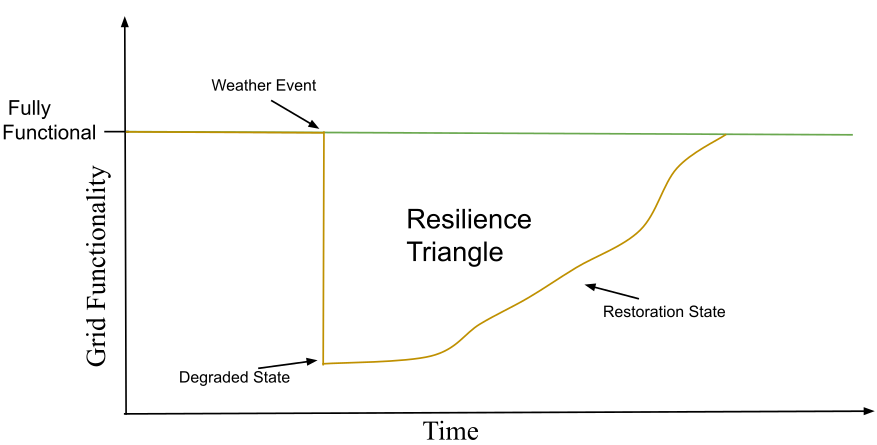
\includegraphics[width=\textwidth]{Resilience Triangle.pdf}
    \caption[Resilience Triangle]{A visual representation of the resilience triangle}
    \label{fig:resiliencetriangle}
\end{figure}
It is apparent that finding the optimal repair sequence to minimize the area of this resilience triangle, and thus the total impact of the event, is a critical field of study. However, it is extremely important that determining this sequence, helps instead of hindering the restoration of the grid \cite{ancona},  and thus it is essential that it does not take a large amount of time. For larger outages, with $n$ grid elements removed, evaluating all $n!$ possible restoration sequences is unfeasible. The majority of the literature attempts to solve this problem for operators in the control room \cite{yan} assuming all of the grid components have already been repaired, such as in \cite{chen}\cite{thiebaux}.  However, there have been various methods proposed which attempt the “Restoration Ordering Problem” as coined in \cite{coffrin2012}. \cite{coffrin2011} proposes injecting precedence constraints while using in a large neighbourhood search in a mixed integer program, including vehicle routing for repair units. \cite{yan} takes the repair crews further, adding in repair crew capacities and trips to the depot in their model. They also include a novel weather dependent repair time for substations as well as ant inspired pheromone trails, speeding up their MIP solution. However, \cite{tan} assumes that crew travel times are small compared to actual repair times after discussion with an industry expert. They use an island by island approach in their solution, prioritizing islands using a soft precedence graph to solve a linear program. However, these MIP based solutions can be difficult to implement and take an uncertain amount of time to complete. \par
 In \cite{nurre}, the grid is simplified to one source and one sink, without losing generality, and treats it as a graph problem, determining which arc to restore next by dividing the amount of residual capacity arc by the time it takes to restore that given arc.  This approach takes its inspiration from Smith’s weighted processing time rule \cite{smith}. Unfortunately, this solution does not appear to schedule a repair sequence on an asset by asset basis. \par
A randomized adaptive decomposition (RAD) method of solving the problem is proposed by \cite{coffrin2012}, where they start with an initial sequence based on basic characteristics of the grid asset (dubbed a utilization heuristic), partition it randomly, and solve the problem for each subsequence individually. They then partition again and repeat, before a stopping condition is reached. They guarantee that their sequence does not worsen after every iteration. \par
Another solution for efficiently decreasing the impact of severe weather events is  by selectively hardening critical grid infrastructure elements structurally to reduce the resilience triangle’s for potential future events. In \cite{chalishazar} this was attempted by simulating earthquakes in Portland and using a component model to determine when grid assets are damaged. They then search for the grid elements which tend to be damaged when a lot of load is lost. Mu et al. \cite{mu} uses  weather and component models to find the probability of failure for transmission lines. They then use that along with the amount of load connected with each line to determine the importance of each line. Braik et al.  \cite{braik} generate tornado events, assuming an EF1 or EF2 magnitude, a set of starting locations and a 45  degree northeastward angle for all tornadoes. They then find the amount of downstream load, assuming a radial network, to determine which lines should be hardened. A machine learning model is used by \cite{hughes2024assessing} to evaluate the effectiveness of resilience improvement strategies such as vegetation management, undergrounding, and structural hardening, in minimizing future outages by utilizing historical outage data for training. These solutions in literature do not utilize the true metric for grid resilience, the area of the resilience triangle, and do not use general weather events which will fully represent the space of possible future hazards. This paper will present a framework for determining the important assets to improve within an entire power network, in responding to a large range of potential tornado events.


\section{Weather Event Creation}
\subsection{Asset Importance Metric}
In order to prioritize the hardening of specific assets, a metric is needed to identify the assets of highest importance. In this paper, the grid assets considered are grid buses and transmission lines. This “importance” metric must be a function of both the assets likelihood of getting damaged by a tornado (or any other extreme weather event), as well as the effect that the asset’s damage on an ensuing outage. There are other key criteria this metric must meet. For instance, it should identify and account for cases where an asset and nearby ones could trigger large outages if they fail simultaneously, as well as the likelihood of such failures occurring together. Additionally, larger outages, caused by more devastating events, are more critical to prevent in order to enhance future resilience. Therefore, these events must be given greater weight.
Given the above criteria, the metric chosen is the following. For each extreme event, and for each asset damaged by that event, the difference in the event’s total impact is found in one case where the asset was damaged, and another assuming the asset was not (as if it had been perfectly hardened). This difference is then summed over each extreme weather event. The metric is presented in equation \eqref{eq:importancemetric} below. 

\begin{equation} 
    I_i = \sum_{j=1}^{n}A_j - A_j^i
    \label{eq:importancemetric}
\end{equation}
Here, $I_i$ is the importance of asset $i$, $n$ is the number of simulated extreme weather events, $A_j$ is the extent of outage $j$, and $A_j^i$ is the extent of outage $j$ assuming asset $i$ was never damaged. In this paper, the extent of the outage is measured as the area of the \textit{Reslience Triangle} in Figure \ref{fig:resiliencetriangle}. \par
The metric is calculated for each asset by completing a Monte Carlo simulation to simulate outages. This entails creating semi-realistic severe tornado events, before determining whether or not grid assets within the tornado’s extent are damaged. After all the assets damaged by the outage are removed, the extent of the event is calculated by finding the area of the resilience triangle. This will be completed via grid network analysis as well as asset repair sequencing, which will be discussed in the following chapter. Then, for each damaged asset, the extent of the outage caused by the tornado will be calculated as if it had never been damaged. \par
This metric was chosen as it is quite simple and yet achieves all of the necessary criteria. It accounts for the likelihood of the asset being hit by an extreme weather event via it having more nonzero elements in the summation of equation \eqref{eq:importancemetric} if it is damaged more during the Monte Carlo simulation. If it is very important for the grids operation, the cost difference in each individual event it is damaged in is likely to be high. As well, if it and another close by asset being damaged simultaneously cause a large outage, this metric will give both assets a large importance if weather events are likely to damage both at the same time. Lastly, events which cause larger outages are more heavily weighted since a simple cost difference is taken instead of averaging the importance over many events.

\subsection{Tornado Model} \label{Tornado Gen}
In creating a tornado model, the TorMC model from \cite{strader} was followed with a few modifications. This model generates a tornado starting location either randomly or from a heatmap, within a pre-determined study region. In this paper, a heatmap provided from NOAA \cite{noaa} for EF2 or higher tornadoes (Figure \ref{fig:noaaheatmap})  was used to determine the starting location . Anthropogenic climate change is likely to change this heatmap as the climate system changes. However, the exact effect of this change on the locations of extreme weather is still uncertain \cite{cheng}. After discussions with an atmospheric scientist who specializes in extreme weather events it was concluded that attempting to determine the change at a grid asset level would be impractical. Consequently, historical data was deemed the most reliable predictor for future weather events. Thus, for other tornado metrics NOAA’s dataset of past tornadoes was used. 
\begin{figure}[ht]
    \centering %center the image
    \includegraphics[width=\textwidth]{noaaheatmap.png}
    \caption[Tornado heatmap from the NOAA website]{Heatmap of past tornadoes from NOAA's website \cite{noaa}.}
    \label{fig:noaaheatmap}
\end{figure}
The NOAA heatmap is structured by having probability of tornado value for various values of longitude and latitude. However, the heatmap is only 45x70, which is not a high enough resolution when simulating weather events at a substation level. To resolve this, SciPy’s interpolate.griddata function was used to refine it to a discrete PDF with a 4000x4000 grid. A 2-D cubic spline interpolation method was specified here. The PDF is then cut to match the study region. \par
When plotting using heatmaps with longitude and latitude, results end up being pole skewed as longitude lines draw closer the further poleward one goes \cite{strader}. Hence, the probability values were normalized by multiplying by the cosine of the latitude. \par
Next, a cumulative probability distribution is calculated for the longitudes. A random value between zero and one is generated, and the CDF is used to map that to a longitude, interpolating between the two nearest grid points in the discrete 4000x4000 PDF. Then, using the closest longitude grid point in the PDF, the conditional CDF is calculated for latitudes given that longitude. Another random value is generated, and a latitude is determined. \par
The results of this process can be seen via the heatmap on the top left of Figure \ref{fig:heatmapresults} below, with he study region being the entirety of the continental United States. This interpolated heatmap closely matches the heatmap provided by NOAA, with the distinct features such as the high probability tornado alley near Mississippi and Tennessee remaining, as well as the low probability region in eastern Kansas and western Missouri. The heatmap created by generated points on the top right of Figure \ref{fig:heatmapresults} was  created using SciPy’s gaussian\_kde function using a 200x200 grid, hence why it is blurrier. The gaussian\_kde function uses kernel density estimation to estimate the PDF of a random variable \cite{scipy}. The bottom figure shows that the 100000 generated points accurately reflect the 4000x4000 heatmap, with a large divergence from what is expected only appearing in locations with few tornadoes. \par
\begin{figure}[ht]
    \centering %center the image
    \includegraphics[width=\textwidth]{heatmapresults.png}
    \caption[Generated and simulated tornado heatmaps over the continental U.S]{Top Left: Heatmap generated after interpolating the NOAA heatmap data. Top Right: Heatmap generated by the generated touchdown points from the Monte Carlo simulation. Bottom: Heatmap created by dividing the top left heatmap by the top right heatmap.}
    \label{fig:heatmapresults}
\end{figure}
Next, unlike \cite{strader}, given a tornado starting location, its magnitude is determined by sampling from the magnitudes of the 50 nearest EF2-or-higher tornadoes to that starting location. This approach was adopted because the heatmaps reveal significant variations in tornado magnitude across different locations. This method avoids placing a high magnitude tornado in a region with no historical precedent of such events preventing the overestimation of grid damages in certain areas. The 50 nearest tornadoes were selected instead of all past tornadoes within a fixed radius to ensure a sufficiently large sample of magnitudes, even in areas with sparse tornado history. \par
Next, to find the angle (or “azimuth” in \cite{strader}) of the tornado, a random angle is selected from all previous tornadoes within the study region of the selected magnitude. A tornado length is then chosen in the same method. Lastly, as in \cite{strader}, a Weibull distribution of tornado widths within the study region is fit for each possible magnitude. Then, a tornado width is sampled from the distribution corresponding to the randomly selected magnitude. The Weibull distribution is used here as the tornado width data from NOAA has a large number of data points at the exact same value, likely due to approximations used when measuring the width. The Weibull distribution allows for a more varied range of width values to be achieved, while fitting the right skewed width data. \par
To test the Weibull distributions, Q-Q plot’s was created to plot the theoretical quantiles calculated from the Weibull distribution against the observed quantiles observed from the data. The quantiles are calculated using filliben’s estimate which finds the expected quantile of a given observed data point given it’s rank in the ordered data set. These Q-Q plots are shown in Figure \ref{fig:WeibullDistribs}.  \par
\begin{figure}[ht]
    \centering %center the image
    \includegraphics[width=\textwidth]{WeibullDistribs.pdf}
    \caption[Fitted tornado width Q-Q plots]{Top Left: Weibull fitted to magnitude 2 tornado width data. Top Right: Weibull fitted to magnitude 3 tornado width data. Bottom: Top left chart zoomed into smaller quantiles. All data is in yards.}
    \label{fig:WeibullDistribs}
\end{figure}
In the figure, the red line represents a linear fit of the data, while the blue line corresponds to $x=y$, which the data would follow if the Weibull distribution perfectly fit the data. In these plots, it is clear to see that many of the observed data values are repeated, such as  unlike the more continuous distribution one might expect with real world weather, justifying the use of the Weibull distribution here.  For the magnitude 3 tornado data, the fit is quite strong justifying that the Weibull is a great choice. For magnitude 2 tornadoes, this is less true, as the Weibull distribution overestimates observed tornado widths at lower quantiles and underestimates them at higher quantiles. However, because the vast majority of the data falls within these lower width values, where the fit is quite strong, the Weibull distribution was deemed appropriate for this use case. This also explains why the fit worsens as width increases, as the more prevalent lower-width data exerts a stronger influence on the fit. \par


Using the selected angle, length, width and the generated starting location, a tornado “box” is formed representing the spatial extent of the tornado path. The substations (and the buses that encompass them) which are within the tornadoes path are found. Additionally, all transmission lines which pass through or are completely within the borders of the tornadoes path are found, and their length within the storm is noted. \par
\subsection{Structural Analysis} \label{FragilityCurve}
Fragility curves have been a key tool in resilience studies to describe the probability of failure of infrastructure in response to extreme weather \cite{serrano2023comprehensive}. These curves describe output the probability of failure of an item given an input on a wide domain of potential loads which could be applied to it. This load could be peak ground acceleration for earthquakes \cite{zekavati2022regional}, wind speed for wind based events \cite{serrano2023comprehensive}, or ice accretion for ice storms \cite{Sheng2023}. As such, fragility curves have been widely used to assess the vulnerability of power system infrastructure \cite{panteli}, with numerous studies dedicated to their development \cite{serrano2023comprehensive}. \par
In this paper, testing the full space of outcomes of outages due to the fragility function for each tornado generated was deemed to be of a lower priority than having a large number of tornadoes generated. For larger study regions, a lower number of tornadoes would cause the heatmap to be poorly explored leading to some system assets being over/under sampled. Thus, the fragility functions were used as thresholds instead of probabilities in this study. \par
For transmission lines, fragility curves from \cite{Watson2024} were used, shown in \ref{fig:TLfragility}. They generated a large distribution of fragility curves using a machine learning model. Taking the middle curve as an average, there is a 50\% chance of failure at a wind load of around 55 m/s. Using the correspondence provided from the American National Weather Service \cite{NWS}, this value corresponds to a EF2 tornado. Hence, as a threshold, transmission lines within the track of a EF2 or higher tornado will be removed. For substations/buses, the complexity of the station causes there to have been little research done on their fragility curves. However, these stations contain smaller towers similar to transmission towers. Hence those towers were used as a proxy. From fragility curves in \cite{dosReis2022}, for an unhardened transmission tower, there is a 50\% chance of failure at wind loads of around 78 m/s. This value corresponds to an EF4 tornado. However, this value is based on a purely wind based load. As discussed in \cite{april}, substation failures tend to be caused by flying debris caused by the tornado. Hence, the threshold for grid substation damage was lowered to an EF3 tornado or higher. \par
\begin{figure}[ht]
    \centering %center the image
    \includegraphics[width=\textwidth]{TLfragility.pdf}
    \caption[Transmission line fragility curves]{Transmission line fragility curves generated by \cite{Watson2024}}
    \label{fig:TLfragility}
\end{figure}
Pure wind (non-tornado) events were also considered in this study. However, even the highest recorded wind gusts, such as the 35 m/s maximum observed in Dallas–Fort Worth over the past 20 years \cite{NWS}, remain well below the 55 m/s threshold associated with a 50\% failure probability in the fragility curve discussed above. Consequently, wind loads were excluded from the analysis. However, climate change may alter this dynamic, as, for example, some RCP8.5 climate simulations project 50-year return level wind speeds to increase by 8–12\% in northern Ontario. Further research is needed to assess how these changes might affect power grid infrastructure. \par

Ice accretion loads were also considered for this paper. For transmission lines, \cite{Xiao2024} presents a 2 axis fragility curve giving probability of failure with respect to wind speed and ice accretion. For transmission towers, \cite{Rezaei} gives failure probabilities with respect to the amount of ice accretion assuming a concurrent wind load of 23 m/s. With these curves, time-series weather data which accounts for extreme values could be used for ice accretion events. Specifically, the Chaine model, which calculates ice thickness on horizontal wires as a function of depth of precipitation, wind speed, drop size and precipitation rate \cite{Sheng2023} is a viable method for modeling ice events. Ice event creation was not conducted in this thesis. However, the asset removals from these events could be easily sent to this paper’s network model in future studies. \par
The time required to repair each grid asset is also important when calculating the area of the resilience triangle. It is difficult to determine this required time, with factors such as the situational awareness of grid operators, coordination of information sharing and the specific asset itself \cite{panteli} influencing it. In this paper, for grid buses this value is assumed to be proportional to the number of transmission lines connected to it, as that scales with the size of the bus and is readily available in the network model. For transmission lines, the repair time is assumed to be proportional to the length of the line within the storm, as the longer the damaged part of the line, the longer it would likely take to repair. For this paper, it is assumed that a line which is within the storm’s extent for one kilometer takes the same amount of time to repair as a grid bus connected to just one line. This is just a temporary representative value and should be refined by using utility repair records for future studies.
\subsection{Synthetic Grids}
To run simulations in this thesis, Texas A\&M’s electric grid datasets \cite{lii} were used. In particular, the 37 bus Hawaii synthetic case was used for testing bus repair sequences and the 6717 bus Texas synthetic case was used for both testing repair sequences and when testing implementation of the grid asset importance framework. Images of the two power grids are shown in Figure \ref{fig:pgrids} below. These synthetic grids do not model the actual grid but do place grid elements such as generators and substations in realistic locations. This realistic model makes them ideal for this work where the geography of the region also impacts factors such as tornado placement.
\begin{figure}[ht]
    \centering %center the image
    \includegraphics[width=\textwidth]{Mock Grids 2.png}
    \caption[Images of Texas A\&M's  Hawaii and Texas mock power grids]{Texas A\&M's  Hawaii (left) and Texas (right) mock power grids \cite{texasam}}
    \label{fig:pgrids}
\end{figure}
\newpage
\section{Outage Repair Sequencing Method} \label{Costfinding}
\subsection{Optimal Power Flow}
Network analysis entails running an optimal power flow (OPF) simulation to determine the manner in which a power system must be dispatched to provide the optimal value for a given variable. Generally, this variable is monetary cost as networks attempt to economically dispatch the available generators. However, after extreme weather events, with potential large scale outages, it becomes critical that the system is dispatched in a manner which maximizes the amount of load delivered. Put the other way, the load shed of the grid must be minimized, defined in equation \eqref{eq:loadshed}.
\begin{equation}
    LS = \sum_{k\in B}P_{D,k} - P_{Del, k}   
    \label{eq:loadshed}
\end{equation}
In equation \eqref{eq:loadshed}, $B$ is the set of buses, $P_{D, k}$ is the power demand at $bus k$, and $P_{Del, k}$ is the power delivered to bus $k$, which is calculated by the OPF. \par
When solving the OPF problem, the AC power flow (AC-PF) equations are generally used to obtain exact solutions. At a given grid bus, these equations are \cite{purchala2005}:
\begin{equation}
    P_k = V_k \sum_{n \in \mathcal{N}_k} V_n \left[ G_{kn} \cos(\delta_k - \delta_n) + B_{kn} \sin(\delta_k - \delta_n) \right]
    \label{eq:ACPFreal}
\end{equation}
\begin{equation}
    Q_k = V_k \sum_{n \in \mathcal{N}_k} V_n \left[ G_{kn} \sin(\delta_k - \delta_n) + B_{kn} \cos(\delta_k - \delta_n) \right]
    \label{eq:ACPFim}
\end{equation}
In these equations, $\mathcal{N}_k$ is the set of buses directly connected to bus $k$, $G_{kn}$ is the conductance of the line between buses $k$ and $n$ and $B_{kn}$ is the admittance. $P_k$ represents the net real power injection at bus $k$, which is the difference between generated and delivered power. If no generator or load is present, $P_k = 0$. \par
Unfortunately, the non-linearity of the AC-PF equations causes them to be extremely computationally expensive to solve. Since this paper involves running a large number of optimal power flow simulations in order to fully explore the space of possible tornadoes, this paper uses the DC optimal power flow (DC-OPF) formulation when running it’s network analysis. DC-OPF involves using the DC power flow (DC-PF) equations which linearize the AC-PF formulas. This linearization ignores the reactive component of the power flow and works under the following conditions \cite{purchala2005}: 
\begin{enumerate}
  \item The voltage at each bus is close to one per unit. This allows the $V_k$ and $V_n$ terms in equation \eqref{eq:ACPFreal} to be set to one.
  \item The transmission line resistances are low relative to the reactance. This allows for the neglect of the $G_{kn}$ term in \eqref{eq:ACPFreal}.
  \item The phase angles of buses directly connected by a transmission line are close. The small angle approximation $\sin(\delta_k - \delta_n) = \delta_k - \delta_n$ can then be used. 
\end{enumerate}
After applying these assumptions, equation \eqref{eq:ACPFreal}  becomes the following:
\begin{equation} 
    P_k = \sum_{ n \in \mathcal{N}_k }\frac{\delta_k - \delta_n}{X_{nk}}
    \label{eq:DCPF}
\end{equation}
Where $X_nk$ is the reactance of the line concecting buses $n$ and $k$. This DC-PF formulation allows for the power flow to be solved in one iteration, vastly improving the time required to compute the power flow. It should be noted however, that these assumptions are not always very realistic. For instance, the reactance to resistance ratio being large may not always be true. Additionally, the per unit bus voltages are likely somewhat variable \cite{purchala2005}. Nonetheless, the DC-PF remains a popular tool in power systems studies \cite{purchala2005} and is used in this paper given the high number of simulations run. \par
Using the DC-PF formulas, an optimal power flow formulation can be formed to minimize the amount of load shed. 
\begin{align}
    \min \quad & \sum_{k\in B}LS_k \\  
    \text{s.t.} \quad & P_{D, k} - LS_k - P_{G, k} +\sum_{ n \in \mathcal{N}_k }\frac{\delta_k - \delta_n}{X_{nk}} = 0 \quad\forall k\in B \label{powerbalance} \\  
                      & \frac{|\delta_{l^+} - \delta_{l^-}|}{X_{l}} \leq P_{l}^{max} \quad\forall l\in \mathcal{L}, \\  
                      & P_{G, k}^{min}\leq P_{G,k} \leq P_{G, k}^{max} \quad \forall k\in B \\
                      & \delta_s = 0
\end{align}	
In this formulation, $LS_k$ and $P_{G, k}$  are the load shed and generation at bus $k$ respectively. $\mathcal{L}$ is the set of transmission lines, with $\delta_{l^+}$ and $\delta_{l^-}$ being the phase at the from and to ends of the line. $P_{l}^{max}$ is the power flow limit through line $l$.   $P _{G, k}^{min}$ and $P _{G, k}^{max}$ are the generator limits for the generator at bus $k$. If bus $k$ is not connected to a generator, both of these are zero. $\delta_s$ is the phase of the \textit{slack bus}, which serves as the angle reference (hence $\delta_s$ = 0) and provides for the ability to balance the power flow throughout the system. \par
In this paper, MATPOWER \cite{zimmerman}., a MATLAB library for power system simulations, was used to solve this optimization problem. MATPOWER uses an interior point solver to conduct the DC-OPF \cite{zimmerman}. The Hawaii and Texas synthetic power grid cases both have casefiles which are importable into MATPOWER. \par

\subsection{Grid Asset Removal Logic}
To assess the impact of outages given a set of damaged grid assets, a mechanism is required to systematically remove and return these assets within the system model. This section outlines the methodology for implementing this process. \par
Given a list of damaged transmission lines and buses, all items in the list were removed from the case file and stored. Additionally, transmission lines connected to damaged buses at either end would no longer be able to carry power and were stored separately. Since they did not require repairs, they could be reinstated as soon as whichever damaged bus (or buses) that was connected to it was repaired and returned to service. \par
Once lines and buses are removed from the system, there is the possibility of \textit{islands} forming, or buses in the system which are disconnected from the main grid. MATPOWER cannot handle these cases as it expects a fully connected grid. To resolve this, a “test\_islanding” function was formed to detect all formed islands, and assign the grid elements. Pseudocode for that function can be found in Appendix~\ref{app:additional-algos}. Afterwards, separate cases are made for each island using its grid elements. If an island does not have a generator, a generator with a power output of zero is added to its case, connected to an arbitrary bus. That bus is also set as the slack bus. If an island does have a generator, but no slack bus, an arbitrary bus with a generator is designated as that islands slack bus. \par
This grid asset removal formulation can lead to two main cases in which the DCOPF can be unsolvable. For one, if the total power demand in an island $\mathcal{I}_i$ is lower than the combined minimum generation of all its generators (i.e equation \eqref{eq:pminfailone} does not hold), the excess power cannot be used, resulting in no feasible solution. This is solved by turning off an arbitrary generator on that island (i.e setting its minimum and maximum power generation to zero) until equation \eqref{eq:pminfailone} holds for that island. 
\begin{equation}
    \sum_{k \in \mathcal{I}_i} P_{G, k}^{min} \leq \sum_{k \in \mathcal{I}_i} P_{D, k}
    \label{eq:pminfailone}
\end{equation}
Another possible failure is for this formulation is as follows. It is possible for the minimum generation of a given bus to be unable to flow through the network due to line power flow constraints, as seen in figure \ref{fig:pminfailtwo}. This was resolved by adding a decision variable (\textit{PMINreduction}) to the OPF which is akin to having a generator which produces negative load next to each existing generator. This requires adding the variable on the left hand side of Equation \eqref{powerbalance}, and settings its maximum to the maximum generation of the generator as well as its minimum to zero. This decision variable is assigned an extremely high cost so that it is only non-zero if that doing so is absolutely necessary to obtain a feasible solution. If any value in \textit{PMINreduction}  is nonzero after running an OPF, the corresponding generators are turned off and the OPF is rerun. This continues until all of \textit{PMINreduction} is zero. \par
\begin{figure}[ht]
    \centering %center the image
    \includegraphics[width=\textwidth]{Pminbroken2.pdf}
    \caption[Potential failure scenario for bus removal programs]{A potential failure scenario for bus removal programs. The lines with red x’s indicate removed transmission lines. The maximum capacity of each line is indicated next to each line. The load demand on the top right bus is zero in this scenario.}
    \label{fig:pminfailtwo}
\end{figure}
\subsection{Asset Sequencing Methods}
As discussed above, it is critical to find the optimal sequence for repairing damaged grid elements which minimizes the area of the resilience triangle. This area, also known as the blackout value or \textit{cost} can be expressed succinctly as the following:
\begin{equation} 
    A=\sum_{i=1}^{n}{P_it_i}
    \label{eq:cost}
\end{equation}
where $A$ is the area of the resilience triangle (or cost), n is the number of damaged assets, $P_i$ is the load outage before the $i$’th asset in the repair sequence is repaired, and $t_i$ is the time required to repair asset $i$. Note that the load outage includes both load that is shed as well as load which is connected to a bus which is currently out of service. This summation can be seen visually in Figure \ref{fig:costfigure} as the total area of the red boxes.  Visually the figure shows that after starting with a large amount of out of service load, repairing grid assets slowly restores some load back into service until the grid is fully operational. It should be noted that in general repairing a grid asset does not necessarily return any additional load to service. \par
\begin{figure}[ht]
    \centering %center the image
    \includegraphics[scale = 0.9]{costfigure.pdf}
    \caption[Cost (blackout value) formula visualized]{In this event, there are 5 damaged grid buses which have been sequenced for repair. On the time axis, the label bus x means that the xth bus in the sequence is currently being repaired at that time. A triangle has been overlaid to show that the cost area somewhat resembles a triangle.}
    \label{fig:costfigure}
\end{figure}
To find the repair sequence which minimizes the cost, an initial first try may be to attempt an exhaustive search of all possible repair sequences. However, to evaluate the cost formula for all sequences of n damaged assets, the number of simulations one would have to run would scale as $n!$. \par
Instead, this process can be run as if one is branching out into all possible sequences of repair. Given $n$ damaged grid elements, attempt scenarios where each of the $n$ elements is repaired first. Then, depending on the outcome of that repair, some scenarios (or in-progress sequences) can be dismissed. Then for each remaining sequence, every remaining grid element is added to that sequence to create a set of repair sequences of length 2. Some of those sequences are then dismissed. This repeats until the sequences reach length $n$, where the sequence with the lowest cost is chosen as the best order to repair the damaged grid assets. Pseudocode for this methodology can be seen below in Algorithm~\ref{alg:pruning}, with code on github at \url{https://github.com/Parveer-B/Get-weather-data}.  This fashion of dismissing in-progress subsequences is akin to the “pruning a tree” \cite{morelato}.

\begin{algorithm}
    \small
    \caption{Repair Sequencing General Form}
    \label{alg:pruning}
    \begin{algorithmic}[1]
    \State \textbf{Input:} 
    \State \quad $n \gets$ number of buses and lines removed
    \State \quad $x \gets$ number of sequences to store
    \State \textbf{Output:} Sequence with lowest cost
    
    \State \textbf{Initialize:} 
    \State \quad $curseq \gets []$ \Comment{Store sequences with current blackout value, time, and criterion}
    \State \quad $newseq \gets []$ \Comment{Store newly generated sequences}
    
    \For{$k = 1$ to $n-1$}
        \If{$k = 1$}
            \For{each element (i.e., bus/line) $j$ from $1$ to $n$}
                \State $toaddseq \gets j$ \Comment{Generate sequence with initial repair of element $j$}
                \State Compute $getoutagedload(toaddseq)$ \Comment{Get load outaged with buses and lines in toaddseq back in the system case}
                \State Append $toaddseq$ to $newseq$ with updated blackout value, and restoration time
            \EndFor
            \State $curseq \gets$ a subset of $newseq$ selected based on some pruning criterion
            \State $newseq \gets []$ \Comment{Reset $newseq$ for next iteration}
            \State \textbf{continue}
        \EndIf
        
        \For{each sequence $seq$ in $curseq$}
            \For{each element (i.e., bus/line) $j$ from $1$ to $n$}
                \If{bus $j$ is not in $seq.sequence$}
                    \State $toaddseq \gets seq.sequence + j$ \Comment{Append element $j$ to $seq.sequence$}
                    \State Compute $getoutagedload(toaddseq)$ 
                    \State Append $toaddseq$ to $newseq$ with updated cost and restoration time
                \EndIf
            \EndFor
        \EndFor
        
        \If{$k \neq (n-1)$}
            \State $curseq \gets$ a subset of $newseq$ selected based on some pruning criterion
            \State $newseq \gets []$ \Comment{Reset $newseq$ for next iteration}
        \Else
            \State $curseq \gets newseq$ \Comment{Keep all sequences}
        \EndIf
    \EndFor
    
    \For{each sequence $seq$ in $curseq$}
        \State Add the remaining grid element to $seq.sequence$
        \State Update cost (assuming load outage after restoration of all damaged buses and lines is 0)
    \EndFor
    
    \State Sort $curseq$ by cost (ascending order)
    \State \Return the sequence with the lowest cost
    
    \end{algorithmic}
\end{algorithm}

To use the above formulation, a methodology must be devised to prune the in-progress sequences. Unfortunately, a truncated cost formula is not ideal for evaluating these sequences as it is only able to include the amount of load shed after that asset is repaired if the time it takes to repair the next asset is known. For an in progress sequence that next asset has not yet been determined. To resolve this, two different mock costs, termed a \textit{restore based} and \textit{load based} mock cost were developed which could assess these in-progress sequences. \par
The load based mock cost (LMC) is similar to the cost except instead of multiplying the time it takes to repair a given asset by the load outage before it is repaired, it is multiplied by the load outage \textbf{after} it is returned to service. It is termed “load based” because the amount of load outage is used in the formula. This formulation was chosen as an option because it includes the effect of restoring the grid asset in its formula. In-progress sequences are considered better if its load based mock cost is lower. Specifically, for an in-progress sequence of length k, which contains buses labelled 1,2,....k in order, the LMC is given as in the equation below. Its value is also shown visually in Figure \ref{fig:LMCFigure} as the area shaded in green:
\begin{equation} 
    LMC =\sum_{i=1}^{k}{P_{i+1}t_i}
    \label{eq:ldmockcost}
\end{equation}

\begin{figure}[ht]
    \centering %center the image
    \includegraphics[scale=0.8]{LMCFigure.pdf}
    \caption[Load based mock cost formula visualized]{The load-based mock cost value is highlighted in green for an ongoing repair sequence that currently includes three buses. The upper edge of the red rectangles represents the current load that is out of service at a given time.}
    \label{fig:LMCFigure}
\end{figure}
The restore based mock cost (RMC) on the other hand explicitly uses the amount of load that repairing a specific grid element brings back into service. This formula is similar Smith’s weighted processing time rule \cite{smith} which has been used incurrent industry practice \cite{tan} with a higher value being better. In this case, the total time was used in the denominator, since using the time it takes to repair the latest asset would often result in cases where in-progress sequences which include the same assets have identical mock costs, regardless of the order in which they were returned to service. This is despite the cost (or blackout value) of those in-progress sequences being different. The restore based mock cost for a sequence of length k is given in Equation \eqref{eq:rbmockcost} and shown visually in Figure \ref{fig:RMCFigure}. In cases where two in-progress sequences may have the same RMC, for example if repairing the assets in the either sequence has not yet returned any load to service, the time it takes to repair the assets in the sequences is used as a tiebreaker.\par
\begin{equation} 
   RMC=\sum_{i=1}^{n}\frac{P_i-P_{i+1}}{\sum_{j=1}^{i}t_j}
    \label{eq:rbmockcost}
\end{equation}
\begin{figure}[ht]
    \centering %center the image
    \includegraphics[scale = 0.8]{RMCFigure.pdf}
    \caption[Restore based mock cost formula visualized]{The restore-based mock cost value is given by the formula for an ongoing repair sequence that currently includes three buses. The upper edge of the red rectangles represents the current load that is out of service at a given time.}
    \label{fig:RMCFigure}
\end{figure}

The mock costs are used to evaluate in-progress sequences in Algorithm~\ref{alg:pruning} lines 15 and 29, and will be compared in section \ref{MCostEval}. However, to decide the number of in-progress sequences kept (i.e saved in $curseq$) in a given iteration, various pruning methods are used. These will be described in the upcoming sections.

\subsubsection{NxGreedy}\label{nxgreedy}
Given a list of of $n$ damaged grid assets, the NxGreedy method involves finding all permutations of these removed grid assets of length $x$. After generating these permutations, the in-progress sequence with the best mock cost is chosen to ’move forward’ (i.e remain unpruned). Afterwards each remaining asset is appended as the next elementin the sequence. The best subsequence is chosen, and the program proceeds greedily until all buses are added. In Algorithm~\ref{alg:pruning} lines 15 and 29, this corresponds to setting $curseq$ equal to $newseq$ if $k < x$, and having curseq only store the best in-progress sequence in newseq if $ k geq x$. The goal of this method is to capture sets of buses of size x or less which only return large amounts of load back into service if they are all repaired. In a purely "greedy" method, where only the best in-progress sequence is kept at each iteration, this could potentially be missed. \par
If $x$ is one, the method becomes purely greedy. Conversely, if $x$ is equal to the number of assets removed ($n$), this method becomes an exhaustive search.\par
The number of power grid simulations (not counting additional islands which may form) run in this method is:
\begin{equation} 
    \sum_{i=1}^{x}\frac{n!}{(n-i)!} + \sum_{i=1}^{n-x}i
    \label{eq:NxGreedysims}
\end{equation}
where $n$ is the total number of assets removed. Note that the final iteration is not simulated as it is assumed that there will be no load shed after all assets are repaired. Instead, all subsequences from the $n-1$th iteration are kept. This is true for all methods.
\subsubsection{Keepx}
The Keepx algorithm adds every remaining grid asset to every existing sequence, before sorting them by their mock cost. It then keeps the top $x$ sequences, proceeds to the next iteration, and repeats the process until all grid assets are back in service. In Algorithm~\ref{alg:pruning} lines 15 and 29, this corresponds to letting $curseq$ equal to the best $x$ sequences in $newseq$ by mockcost. \par
With this approach, the total number of simulations is given by:
\begin{equation} 
    n + \sum_{i=2}^{n}x*(n-i+1)
    \label{eq:Keepxsims}
\end{equation}
If $x = 1$, this method becomes greedy.
\subsubsection{Closecostx\%}
Closecostx\% works almost exactly the same as Keepx. However instead of keeping the best x sequences by mock cost, all sequences in $newseq$ within x\% of the best mock cost are stored in $curseq$. This approach does not have a set number of simulations, and thus the time it takes to complete is more variable than the others.

\subsubsection{PerxGreedy}
PerxGreedy is very similar to NxGreedy. However, after greedily picking the best sequence at iteration $k=x$, the method once again adds all permuations of length x of the remaining grid assets to the chosen subsequence. This continues every x iterations. This is akin to setting $curseq$ equal to $newseq$ in Algorithm~\ref{alg:pruning} lines 15 and 29 if $k\%n \neq 0$, and storing only the best sequence by mockcost in $curseq$ if $k\%n \equiv 0$. The goal of this method is similar to that of NxGreedy. However instead of just finding sets of buses which restore a lot of load when repaired together at the \textit{start} of the sequence, this method can find these sets at any point in the sequence at the cost of additional computation time.

\subsection{Method Evaluation}
\subsubsection{Storm Travel Line}
To evaluate mock costs and pruning methods, asset damaging fake disasters must be generated. In this section, it was assumed that only grid buses were damaged. To remove buses a “storm travel line” was used as a mechanism to mock a path that astorm might travel. This storm travel line entails removing a bus at random. Then usingthe lines connected to that bus, an adjacent bus is chosen to remove. Using the set of busesadjacent to both buses another bus was selected, repeating the process until a predetermined number of buses ($n$) is removed. Additionally, in this chapter, the load demand on the Texas and Hawaii cases was scaled so that the maximum allowable power generated by the system's generators were close to the load demand. This was done to prevent "wasted" cases where there was minimal load outage. For the Texas case, this load scaling was set at 1.25x, while for the Hawaii case this was 1.2x. These values were chosen because increasing the load scaling slightly beyond these values resulted in load shedding, even without any buses being removed.

\subsubsection{Mock Cost Evaluation} \label{MCostEval}
The two mock costs were compared by generating 100 "storms" via the storm travel line method in the Hawaii mock grid case with 5 buses removed. The repair sequences were found using Algorithm~\ref{alg:pruning} and both mock costs were used individually throughout the algorithms process in lines 15 and 29 for a given event. The same events were used for both mock costs. Using a purely greedy (i.e N1Greedy) method for pruning repair sequences, the LMC resulted in finding sequences with a blackout value which were 12\% higher than that when using the restore based mock cost on average. Of the 100 storms, the RMC found sequences with a lower blackout value than the LMC 88 times, and found sequences with the same cost 6 times. The LMC was only better than the RMC 6 times. Using the Keepn method (i.e. Keep5 in this case), the LMC had an average cost which was 1.9\% higher than the RMC. Here, the LMC was better only 3 times, while the RMC was better 41 times. \par
150 scenarios of the Hawaii case were then run with 3 buses removed. Here, was Keepn was not tested as all in-progress sequences are kept in the $n-1$th (i.e 2nd) iteration causing Keepn to be an exhaustive search here. Once again, the same storms were used to test both mock costs Using the greedy method, the LMC was 4.3\% worse than the RMC, and it was only better in 5 of the 150 scenarios. It was worse in 63 of the 150 simulations. \par
These results demonstrate that the RMC is likely better than the LMC. This can be attributed to the fact that when a sequence begins, the load remaining is likely significantly larger than the load that is returned to service simply by putting one bus back in service. Thus, at the start the actual effect of repairing a bus probably has very little effect on the LMC. The simulation will then likely simply choose the bus which is the fastest to repair, regardless of how much load it restores. With the RMC, the amount of load restored is used directly. Consequently, at the start of the sequence it will prioritize repairing buses which restore the most load as well as taking the least time to repair. \par
Nonetheless, there are cases where the load-based mock cost proves more effective. For instance, there can be a scenario where two buses are damaged but can be quickly restored with neither bus restoring any load individually. However, the restoration of both together may restore a significant amount of load. In this situation, the restore based mock cost with the greedy method will instead choose to restore a bus that restores some amount of load, even if that bus takes a lot longer to restore. Despite this, the restore based mock cost is the only one used for the rest if this paper as it is better in the majority of cases.

\subsubsection{RAD}
These tree pruning mechanisms were tested against the RAD method proposed in \cite{coffrin2012} and described in Section \ref{LitReview}. In this paper, random partitioning was implemented such that each partition contained at least two elements, with a maximum partition size being half  the number of buses out. This maximum limit was chosen to ensure that solving the ordering problem for the partitions remained computationally feasible. The partitioning process involved selecting a random number between two and the maximum size, forming a partition, and repeating until all buses were assigned. Both exhaustive search and a purely greedy approach were tested for solving the ordering problem for a partition. If the exhaustive search was used, the maximum partition size was set at 4 to not have an overly long computation time.  The stopping condition was defined as the entire sequence maintaining the same cost for $x$ consecutive iterations or 30 iterations total, whichever comes first. \par

Four ways of generating initial sequences (or utilization heuristics) were tested. In \cite{coffrin2012} they found a sequence by the sorting buses by the amount of power flow through them. In this paper, this was done by running a DC-OPF to solve the economic dispatch problem and summing the outward flow from each bus. The power flow through each bus divided by the time it takes to repair that bus was also tested. As well, \cite{tan} states that repair sequencing by sorting by the load of each bus and by the load of each bus divided by time is used in practice. Both of these were also tested.

These initial sequences were tested in three different trials, with the partition ordering problems solved optimally. The first and second trial both involved 150 "storms" generated via the storm travel line with 5 buses removed in the Hawaii case. The third trial was 150 storms with 8 buses removed in the Hawaii case. For all three of these trials, the stopping condition was set as the sequence maintaining the same cost for 3 consecutive iterations. As well, the same storms were used for each heuristic. The results of this testing are in Table \ref{tab:rad_results}, and the average time to run each storm  for each trial is given in Table \ref{tab:rad_times}. The values in the table indicate the percentage by which the average cost of each method is lower than the baseline cost. In other words, a value of 1\% in the table indicates that that the average cost of that method is 1\% lower than the baseline cost. The baseline  was arbitrarily set to be the utilization heuristic which sorts by the amount of load. 

\begin{table}[ht]
    \centering
    \begin{tabular}{|c|c|c|c|c|}
        \hline
        & \makecell{Sort by \\ Load} 
        & \makecell{Sort by \\ Load / Repair Time} 
        & \makecell{Sort by \\ Power Flow} 
        & \makecell{Sort by \\ PF / Repair Time} \\
        \hline
        \textbf{5 buses out} & 0 & -0.35\% & -0.29\% & -1.63\% \\
        \hline
        \textbf{5 buses out (v2)} & 0 & -0.34\% & -0.59\% & -1.16\% \\
        \hline
        \textbf{8 buses out} & 0 & -1.31\% & -0.55\% & -1.19\% \\
        \hline
    \end{tabular}
    \caption{Comparison of RAD utilization heuristic costs}
    \label{tab:rad_results}
\end{table}

\begin{table}[ht]
    \centering
    \renewcommand{\arraystretch}{1.2} % Adjusts row height for better spacing
    \begin{tabular}{|c|c|c|c|c|}
        \hline
        & \makecell{Sort by \\ Load} 
        & \makecell{Sort by \\ Load / Repair Time} 
        & \makecell{Sort by \\ Power Flow} 
        & \makecell{Sort by \\ PF / Repair Time} \\
        \hline
        \textbf{5 buses out} & 7.54 & 7.66 & 8.26 & 6.91 \\
        \hline
        \textbf{5 buses out (v2)} & 7.58 & 7.41 & 8.15 & 7.16 \\
        \hline
        \textbf{8 buses out} & 45.17 & 48.33 & 47.11 & 44.77 \\
        \hline
    \end{tabular}
    \caption{Comparison of RAD utilization heuristic run times}
    \label{tab:rad_times}
\end{table}

From the results it is clear that simply sorting the buses by the amount of load connected to them performs the best. In terms of run time, this method is on the same order as the other ones, and is only consistently slower than starting by sorting by power flow/time (which is the worse utilization heuristic). Thus, for RAD in this paper, the initital sequence of buses is determined by sorting by the amount of load connected to each one.

\subsubsection{5-Bus Pruning Method Evaluation} \label{5buseval}

In a first round of testing, the N1Greedy, N2Greedy, Closecost1\%, Keepn, Exhaustive Search, Closecost2\% and Keepn/2 methods were tested, with $n$ being the number of buses damaged. In Keepn/2 uses the Keepx method with $x = \lfloor \frac{n}{2} \rfloor$  These methods were first tested in the Texas case with 5 buses removed. There were 150-175 storms simulated for each method, and the same storm was \textbf{not} used for each method here. However, N1Greedy was used every time as a baseline. 'Percentage Better than N1Greedy' refers to the percentage by which the blackout value of the sequence obtained using that method is lower than the one found by N1Greedy. This percentage difference is averaged over all the storms. On the right side of  Figure \ref{fig:Texas5busr1}, the x-axis gives the average that percentage over the first $x$ storms. This was used to test the convergence of the results. The average percentage better than N1Greedy over all the storms simulated for that method is shown on the left of Figure \ref{fig:Texas5busr1}.

\begin{figure}[ht]
    \centering %center the image
    \includegraphics[scale = 0.24]{Texas5busr1.pdf}
    \caption[Initial Testing - 5 buses removed, Texas Case]{Various pruning methods tested for different storms in the Texas case. N1Greedy is used as a baseline.}
    \label{fig:Texas5busr1}
\end{figure}

Several observations can be made from the graph above. The first notable point is that Keepn appears to outperform the exhaustive search. This is due to the algorithms being conducted on different cases. As additional storms are simulated, Keepn will likely fall below it. Nonetheless, this result demonstrates that Keepn is consistently very close to finding the optimal restoration sequence while operating in roughly one-third of the time. \par
Another key observation is that N2Greedy appears to perform the worst among these methods. A discernible trend can be observed where an increase in computation time corresponds to improved accuracy. This trend can be visualized by a "line" passing through the points for Ng1reedy, Closecost1\%, Closecost2\%, Keepn/2, and Keepn. However, N2Greedy exceeds the processing time of Closecost2\% while yielding less accurate results. \par
Finally, the cost results are relatively consistent across the different pruning methods. Ngreedy1 is only about 1.2\% worse than the exhaustive search, suggesting that it is an option to save time without sacrificing much efficacy. \par

The convergence data shows that these results were able to convergerge within the 150-175 storms demonstrating that the uncertainty on the results is likely quite low.\par

The same test was run on the Hawaii case. This time 500 storms were run for each method, with the same storms used for each. More storms were run on the Hawaii case since the smaller case file generates solutions faster. Results are shown in Figure \ref{fig:Hawaii5busr1}.

\begin{figure}[ht]
    \centering %center the image
    \includegraphics[scale = 0.24]{Hawaii5busr1.pdf}
    \caption[Initial Testing - 5 buses removed, Texas Case]{Various pruning methods tested for different storms in the Hawaii case. N1Greedy is used as a baseline.}
    \label{fig:Hawaii5busr1}
\end{figure}
In these cases, it is clear that Keepn outperforms the other options and is quite close to optimal on average despite taking a third of the time. Additionally, N2Greedy performs worse than N1Greedy despite taking more time to compute. Following these results, N1Greedy and Keepn were chosen for further testing. These were chosen since N1Greedy is a fast and less accurate method, while Keepn takes longer computationally while being quite close to finding the optimal solution in cases with 5 buses removed. While Closecost1\% and Closecost2\% are slightly better than N1Greedy with very little variation in the average time to complete, the performance increase was not deemed to be high enough to compensate for the uncertain solution time of these methods. However, Keepn/2 is still a possible option to balance computational time and efficacy if needed. A summary of the performance based can be seen in Table \ref{tab:r1results}. \par

\begin{table}[ht]
    \centering
    \renewcommand{\arraystretch}{1.2} % Adjust row height for better spacing
    \begin{tabular}{|c|c|c|}
        \hline
        \textbf{Method} & \makecell{\% Worse than Optimal, \\ Hawaii} & \makecell{\% Worse than Optimal, \\ Texas} \\
        \hline
        N1Greedy & 1.43\% & 1.07\% \\
        \hline
        N2Greedy & 1.71\% & 0.88\% \\
        \hline
        CC1\% & 1.18\% & 0.68\% \\
        \hline
        CC2\% & 1.11\% & 0.61\% \\
        \hline
        Keepn & 0.13\% & -0.05\% \\
        \hline
        Keepn/2 & 0.67\% & 0.42\% \\
        \hline
    \end{tabular}
    \caption{Comparison of algorithm performance relative to optimal}
    \label{tab:r1results}
\end{table}

The efficacy of the methods seems to follow approximately the same ordering in either case, with only N1Greedy switching with N2Greedy when going from Hawaii to Texas. However, there is a larger variability in the effectiveness of the each method in the Hawaii case. For example N1Greedy is 1.43\% worse than optimal in the Hawaii case, and only 1.07\% worse than optimal in the Texas case. This is likely beause the smaller scale of the Hawaii system causes the removed buses to have had a larger impact on the performance of the network with the Texas case having more options to make up the lost load. Thus, there is a larger variability in the cost of different restoration solutions, leading to worse results on average relative to an exhaustive search. \par

\subsubsection{10-Bus Pruning Method Evaluation}
RAD, Per2Greedy and Keepn were then tested relative to N1Greedy. Four different variations of RAD, the optimal and greedy solving of the partition ordering problem paired with a stopping condition of three and six consecutive sequences (denoted by "same" in \ref{fig:Hawaii10busr2}) were used. In this test, ten buses were removed on the Hawaii case, with 288 storms run. These storms were the same for each method. Ten buses were tested here to allow for a larger number of allowable partitions for the RAD algorithm based on the constraints discussed above. With five buses removed, there are only three allowed partitions with those stipulations making RAD less effective. Results are shown in \ref{fig:Hawaii10busr2}.

\begin{figure}[ht]
    \centering %center the image
    \includegraphics[scale = 0.24]{Hawaii10busr2.pdf}
    \caption[Second Testing Set - 10 buses removed, Hawaii Case]{Various pruning methods and RAD tested for different storms in the Hawaii case. N1Greedy is used as a baseline.}
    \label{fig:Hawaii10busr2}
\end{figure}

The convergence chart shows that the solutions have converged and thus the chart results are decently accurate. The greedy sorting of partitions in RAD performs worse than greedily pruning in-progress sequeunces, while taking double and triple the time. Additionally, Radoptsame3 performs worse than Per2Greedy while taking double the time, while Radoptsame6 performs worse than Keepn while taking almost double the time. Thus, for storms with ten or less assets removed these pruning methods should be used instead of RAD. Additionally, it should be noted that Keepn's efficacy increased from 1.3\% better than N1Greedy with five buses removed in the Hawaii case to 3\% better. This was expected as the number of solutions scales up drastically as the number of buses removed increases, and thus it is more likely that N1Greedy prunes a critical subsequence which Keepn keeps. Additionally, with 10 buses removed, there is likely a larger variance in the cost of different possible repair sequences, leading to a larger variance in the efficaccy of different solutions. It is possible that at ten buses removed, Keepn is now significantly worse than an exhaustive search. Unfortunately, conducting that test by finding all $10! = 3628800$ possible sequences was determined to be unfeasible due to time and storage constraints. \par

As a final test, Keepn, Per2Greedy and N1Greedy were tested with 10 buses removed in the Texas case. This was conducted to measure the approximate consistency of the results across different grid networks. 836 storms were run, with the same storms for each method. Results are in \ref{fig:Texas10busr2}.

\begin{figure}[ht]
    \centering %center the image
    \includegraphics[scale = 0.24]{Texas10busr2.pdf}
    \caption[Second Testing Set - 10 buses removed, Texas Case]{N1Greedy, Per2Greedy and Keepn tested for different storms in the Texas case. N1Greedy is used as a baseline.}
    \label{fig:Texas10busr2}
\end{figure}

The relative ordering of the effectiveness and time required for Keepn, Per2Greedy and N1Greedy is similar here as in \ref{fig:Hawaii10busr2}. Interestingly the percentage difference between Keepn and Per2Greedy relative to N1greedy when switching from the Texas to the Hawaii case actually decreases, with Keepn being about 3\% better than N1Greedy in the Hawaii case and over 3.5\% better in the Texas case. \par

\subsubsection{Summary of Results}
In summary, the pruning methods have been shown to be an effective way to find bus repair sequences in storms with less than 10 buses removed. With 5 buses removed, Keepn is extremely close to finding the optimal solution, and even a purely greedy method in N1Greedy is only 1 to 1.5\% worse than the optimal solution. With 10 buses removed, the pruning methods outperform the RAD method from \cite{coffrin2012}, although their performance relative to a full exhaustive search is unknown. In general, the Keepn method appears to have the best performance at the cost of computational time, while the N1Greedy method is a much more time-efficient method, albeit with a slight decrease in efficacy. For methods which balance computational time and efficacy, Keepn/2 and Per2Greedy have presented themselves as viable alternatives.
\newpage

\section{Bus Importance Simulation}
\subsection{Simulation Setup}
This section will outline the bus importance simulation run as a proof of concept for the above's methodology. Tornadoes will be generated as discussed in Section \ref{Tornado Gen}, and buses and transmission lines will be removed as described in Section \ref{FragilityCurve}. Afterwards power system simulations will be run using methods in Section \ref{Costfinding}. After running a large number of tornadoes, an asset importance metric will be calculated. \par
For this simulation, the Texas system case will be used, with bus and transmission line locations being provided by the casefile. For tornado generation, the heatmap region was cut into a rectangle which encompasses the entire state of Texas, so that tornadoes would only be generated in that area. The NARVAL supercomputer, a computing cluster located at the École de technologie supérieure in Montréal \cite{NARVAL} was used to complete these simulations. The cluster has a AMD EPYC 7532 CPU which has a 2.40 GHz clock speed. \par
When generating magnitude 5 tornadoes, tornado angle, width and length data will additionally be sampled from surrounding states (Louisiana, Oklahoma, Arakasas and New Mexico) in order to have a wider range of possible generated tornado shapes. Currently, there are only six recorded magnitude five tornadoes in Texas, a number that increases to 18 if surrounding states are included. \par
Unfortunately, simulating the DC-OPF for the Texas case takes approximately 3 seconds on the NARVAL supercomputer. To compute the asset importance metric for a tornado that removes $k$ buses, we must determine the area of the resilience triangle (or cost) for two cases: (1) the event where $k$ buses are removed and (2) separate scenarios where each of those $k$ buses remains undamaged while the others are removed. This requires an additional $k$ simulations for cases with $k-1$ buses removed. Using formula \ref{eq:Keepxsims}, which determines the number of simulations required to compute the cost of an event with $n$ buses removed, we can calculate the total number of power grid simulations needed to determine the asset importance metric via the Keepn method for a tornado that removes $k$ grid elements. This number of simulations can then be converted to the approximate time required to complete the power system simulations for that one tornado on the NARVAL supercomputer. This is presented in Figure \ref{fig:Keepnnumsims}. \par

\begin{figure}[ht]
    \centering %center the image
    \includegraphics[width=\textwidth]{Keepnnumsims.pdf}
    \caption[Time required to find importance metric with Keepn]{The time required on NARVAL to find the asset importance metric with the Keepn pruning method for a storm with n assets damaged. The red line represents over a day to complete, while the green line is 6 hours (deemed the maximum "reasonable" time to complete the event).}
    \label{fig:Keepnnumsims}
\end{figure}

From Figure \ref{fig:Keepnnumsims}, it is clear that the time required for the metric to be calculated becomes unreasonable extremely quickly. Passing six hours with after $n = 10$, and one day after $n = 15$. Conversely, if N1Greedy is used, the results are as follows in Figure \ref{fig:Keep1numsims}. \par


\begin{figure}[ht]
    \centering %center the image
    \includegraphics[width=\textwidth]{Keep1numsims.pdf}
    \caption[Time required to find importance metric with N1Greedy]{The time required on NARVAL to find the asset importance metric with the N1Greedy pruning method for a storm with n assets damaged.}
    \label{fig:Keep1numsims}
\end{figure}

This is a bit more reasonable with it being reasonable below $n=22$ and only taking over a day at about $n=35$. However some storms, partiularily those through downtown cores such as Dallas and Houston can often take out upwards of 50 grid assets. If $n=60$, even with the purely greedy method, it would still take about five days to calculate the importance metric for that single storm. \par
Another possibility is to vary the method depending on how many assets are damaged. For example, if Keepn is used for $n\leq8$, Keepn/2 is used for $9 \leq n \leq 12$, Keepn/4 (i.e Keepx  with $x = \lfloor \frac{n}{4} \rfloor$) for $13 \leq n \leq 15$ and greedy otherwise, the graph becomes that in \ref{fig:Keepvariednumsims}.This formulation is somewhat counterintuitive as methods such as Keepn get better relative to N1Greedy if more assets are removed. However, here it is N1Greedy that is being used in situations with more assets damaged. Nonetheless, it ensures that simulation times stay reasonable for as long as possible when using pruning methods.\par


\begin{figure}[ht]
    \centering %center the image
    \includegraphics[width=\textwidth]{Keepvariednumsims.pdf}
    \caption[Time required to find importance metric with various methods]{The time required on NARVAL to find the asset importance metric for a storm with a combination of pruning methods based on the number of assets damaged.}
    \label{fig:Keepvariednumsims}
\end{figure}

In this paper, due to the short timelines of the EngSci thesis project, N1Greedy was used as the pruning method for all storms. To run the simulation, storms were generated in batches of 200, and 200 NARVAL jobs were submitted to run power system simulations and calculate the bus importance metric for each batch. Each batch was given a week (the NARVAL job time limit) to complete as many storms as possible. Data was saved after every 1000 storms within a batch to prevent data loss. It should be noted that this implicitly does affect the importances of assets in high density areas, as those batches which may end up with a lot of storms in those areas will likely take longer to run, and thus less importance metrics for storms in those areas will be calculated.

\subsection{Simulation Results}



\newpage
\bibliographystyle{unsrt} % You can use other styles like 'unsrt', 'alpha', etc.
\bibliography{references}
\newpage 
\appendix 
\section{Other Algorithms}
\label{app:additional-algos}
\begin{algorithm}
    \caption{Island Detection}
    \scriptsize
    \begin{algorithmic}[1]
    \Function{TestIslanding}{branches, buslist}
        \State foundBuses $\gets$ empty list
        \State islands $\gets$ empty list
    
        \Comment{Check for empty branches}
        \If{branches is empty}
            \For{each bus in buslist}
                \State Append bus to islands
            \EndFor
            \State \Return
        \EndIf
    
        \Comment{Check for single branch case}
        \If{size(branches, 1) = 1}
            \State Append \{branches[1,1], branches[1,2]\} to islands
            \For{each bus in buslist}
                \If{bus is not in islands[1]}
                    \State Append bus to islands
                \EndIf
            \EndFor
            \State \Return
        \EndIf
    
        \Comment{General case}
        \For{each bus in buslist}
            \If{bus is in foundBuses}
                \State Continue
            \Else
                \State curIter $\gets$ \{bus\}
                \State island $\gets$ \{bus\}
                \State Append bus to foundBuses
    
                \While{true}
                    \State nextIter $\gets$ empty list
                    \For{each bus in curIter}
                        
                        \Comment{Find branches where bus is on the "from" end}
                        \State adjBranches1 $\gets$ branches where bus on the from end of it
                        \For{each branch in adjBranches1}
                            \If{bus on "to" end of branch not in nextIter and not in foundBuses}
                                \State Append bus on "to" end of branch to nextIter
                            \EndIf
                        \EndFor
                        
                        \Comment{Find branches where bus is on the "to" end}
                        \State adjBranches2 $\gets$ branches where bus is at the "to" end
                        \For{each branch in adjBranches2}
                            \If{bus on "from" end of branch not in nextIter and not in foundBuses}
                                \State Append bus on "to" end of branch to nextIter
                            \EndIf
                        \EndFor
                        
                    \EndFor
    
                    \If{nextIter is empty}
                        \State Append island to islands
                        \State \textbf{break}
                    \EndIf
    
                    \State curIter $\gets$ nextIter
                    \State Append nextIter to island
                    \State Append nextIter to foundBuses
    
                \EndWhile
            \EndIf
        \EndFor
    \EndFunction
    \end{algorithmic}
\end{algorithm}

\end{document}